\documentclass[journal]{IEEEtran} % use the `journal` option for ITherm conference style
\IEEEoverridecommandlockouts
% The preceding line is only needed to identify funding in the first footnote. If that is unneeded, please comment it out.
\usepackage{cite}
\usepackage{amsmath,amssymb,amsfonts}
\usepackage{algorithmic}
\usepackage{graphicx}
\usepackage{textcomp}
\usepackage{xcolor}
\graphicspath{ {./images/} }
\def\BibTeX{{\rm B\kern-.05em{\sc i\kern-.025em b}\kern-.08em
    T\kern-.1667em\lower.7ex\hbox{E}\kern-.125emX}}
\begin{document}

\title{LiDAR Object Tracking with Hardware Acceleration}


\author{%%%% author names
    \IEEEauthorblockN{McCain Boonma}\\% first author
    \IEEEauthorblockA{\textit{Northeastern University, Boston, USA}}\\% first affiliation
    \IEEEauthorblockA{boonma.m@northeastern.edu}
}

\maketitle

\begin{abstract}
This project explores the implementation of hardware acceleration for real-time processing and analysis of Light Detection and Ranging (LiDAR) data using a Field-Programmable Gate Array (FPGA). A custom hardware implementation of the Density-Based Spatial Clustering of Applications with Noise (DBSCAN) algorithm is developed and evaluated, demonstrating significant speedup and reduced resource utilization compared to the software implementation. A constant velocity Kalman filter is used to track clusters over time, with graphical output for visualization of the clustering and tracking results. The project also identifies potential enhancements to the system, such as improving latency, increasing resolution, and transitioning the Kalman filter to hardware. Overall, this project demonstrates the effectiveness of FPGA-based hardware acceleration for real-time LiDAR data processing and analysis, with potential for future optimizations and improvements.
\end{abstract}

\section{Introduction}
Light Detection and Ranging (LiDAR) sensors are widely used in various applications, including autonomous vehicles, robotics, and environmental monitoring. These sensors generate large amounts of data that require real-time processing to detect and track objects within their field of view. This paper presents an efficient solution for real-time processing and analysis of LiDAR data, leveraging FPGA-based hardware acceleration to perform clustering and a Kalman filter for object tracking. The proposed approach employs a number of hardware optimizations in the point clustering operation, resulting in significant improvements in overall performance. The processed data is visualized using polar plots , providing a clear representation of the raw LiDAR data and the identified clusters.

\section{System Overview}
This inclusive system (Fig \ref{fig:sysOverview}) includes LiDAR data collection, point clustering, and object tracking. The primary focus of this paper is the clustering algortihm implemented on the FPGA programmable logic via an overlay and the object tracking using a Kalman filter implemented on the FPGA processing system. 

\begin{figure}[h]
  \centering
  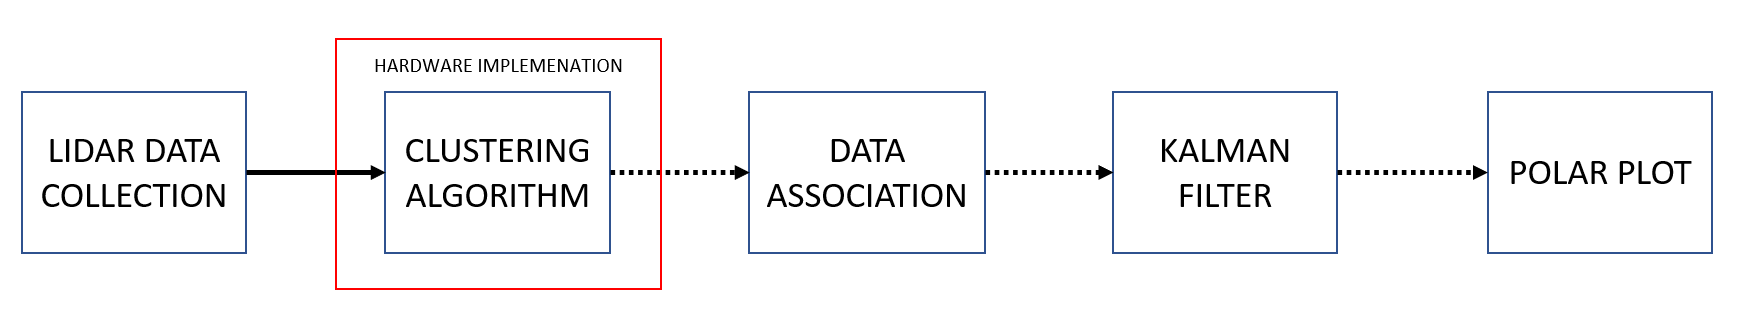
\includegraphics[width=0.5\textwidth]{sysOverview}
  \caption{System Overview}
  \label{fig:sysOverview}
\end{figure}

\subsection{LiDAR Data Collection}

The sensor's coordinate system is defined such that 0\textdegree originates from the center of the sensor assembly towards the LiDAR sensor's motor, with data collected in the clockwise direction (as shown in Fig. \ref{fig:polarLiDAR}). The sensor is connected to the processing system of the PYNQ Z2 via a USB port.

\begin{figure}[h]
  \centering
  \includegraphics[width=0.35\textwidth]{polarLiDAR}
  \caption{LiDAR Sensor Coordinate System Definition}
  \label{fig:polarLiDAR}
\end{figure}

 To control the LiDAR sensor and collect LiDAR data, the PyLidar3 library is utilized, which is a python 3 package. The LiDAR sensor is capable of a typical angle resolution of 0.50\textdegree at 7 Hz, but due to software limitations, the PyLidar3 library provides a resolution of only 1\textdegree regardless of the frequency. The collected data is returned in the form of a dictionary, comprising of 360 degrees of angle and corresponding distances in millimeters.\\


\subsection{Hardware Accelerated Point Clustering}

The point clustering operation was implemented on the programmable logic of the FPGA using an Overlay. To achieve this, the point clustering algorithm was developed in Vitis High-Level Synthesis (HLS). The LiDAR data is transferred from the FPGA processing system to the programmable logic through an AXI Stream interface, while the clustered data is transferred via a separate AXI Stream interface. The implemented clustering algorithm is based on the Density-Based Spatial Clustering of Applications with Noise (DBSCAN) algorithm, which is commonly utilized in LiDAR point clustering applications.\\

he clustering algorithm utilized in the proposed LiDAR object tracking system is based on the Density-Based Spatial Clustering of Applications with Noise (DBSCAN) algorithm. The DBSCAN algorithm takes three parameters: an array of distance data, the number of data points, and the maximum distance between two points in the same neighborhood (epsilon, $\epsilon$).

The DBSCAN algorithm starts by iterating over all the points in the input data array. For each unvisited point, the algorithm finds all its neighbors within a distance of $\epsilon$ and adds them to a cluster. The algorithm then expands the cluster by adding all reachable neighbors of each point in the cluster. The algorithm stops when no more points can be added to the cluster.

The distance calculation used in the DBSCAN algorithm takes into account the angle between the LiDAR points, which are represented as distances in an array. Given two points $p_1$ and $p_2$ in the array, the distance calculation between them is as follows:

\[
distance = \sqrt{(p_{1,x} - p_{2,x})^2 + (p_{1,y} - p_{2,y})^2}
\]

Where $p_{1,x}$ and $p_{2,x}$ are the distances of $p_1$ and $p_2$ from the LiDAR sensor along the horizontal axis, and $p_{1,y}$ and $p_{2,y}$ are the distances of $p_1$ and $p_2$ from the LiDAR sensor along the vertical axis. The distance calculation also involves converting the angles of the LiDAR points to radians, and using the sine and cosine functions to compute the horizontal and vertical distances respectively.

The implemented DBSCAN algorithm in the code snippet takes an array of distance data, the number of data points, and the maximum distance between two points in the same neighborhood (epsilon, $\epsilon$) as input. The algorithm iterates over all the points in the input array, finds all the neighbors of each unvisited point, and creates a new cluster if the point has enough neighbors. The algorithm then expands the cluster by adding all reachable neighbors, and continues until no more points can be added to the cluster.

After the raw LiDAR data set has been clustered, a Python helper function calculates each cluster's centroids and stores the clusters as centroid angle, centroid distance, and cluster size. 

%-----------------------------------------------------------------------------------------------------------------------------------------------------------------------------------------------------------------------------------------------
\subsection{Data Association - Scoring Algorithm}

In this particular application, the noise generated by the LiDAR sensor is significant and the size and location of the clusters varied significantly. Therefore, a robust data association algorithm was needed to match clusters from a previous frame in the current frame. To achieve this, a scoring algorithm was employed to match clusters between frames using the predictions from the Kalman filter.

In the first iteration, the master list was initialized by clustering the first dataset and storing it in the format of cluster centroid angle, cluster centroid distance, and cluster size. Each cluster was assigned a unique ID and stored in a master list. In subsequent iterations, a list of the current clusters, represented by their centroid and size, was generated. The data association algorithm iterated over each cluster in the master list and calculated a score against each cluster in the current frame's clusters. The current cluster with the lowest score was matched with the predicted state of the cluster under test from the Kalman filter.

The score was an aggregate score between the size of the cluster and the polar euclidean distance (PED), which is given by the following equation:

\[
\text{PED} = \sqrt{r_1^2 + r_2^2+2r_1r_2cos(\Delta\theta)}
\]

The aggregated score was calculated by multiplying the difference in cluster size and euclidean distance with double the weight assigned to the PED, as shown in the following equation:

\[ 
\text{Score} = \Delta \theta * 2  \text{PED}
\]

Due to the noise, it was possible for the master list to fluctuate in size. The data association algorithm took this into account. If there were more clusters in the current cluster list than in the master list, then the clusters not matched with a cluster from the master list were assigned a new unique ID. On the other hand, if there were more clusters in the master list than in the current cluster list, then the data association algorithm found and removed the excess clusters from the master list. The data association function matched each cluster in the master list, and in this case, multiple clusters in the master list could be matched to the same cluster from the current list. The data association function removed the matched clusters with the highest score, i.e., the worst fit.

The data association function replaced the master list with the newly updated lists. Each matched cluster retains the unique ID of the cluster the scoring algorithm determined was the best fit based on the cluster size and euclidean distance between the centroids. The Kalman filter is then updated with the matched cluster's measurements, improving the accuracy of its predictions in subsequent iterations.

%-----------------------------------------------------------------------------------------------------------------------------------------------------------------------------------------------------------------------------------------------

\subsection{Kalman Filter for Cluster Tracking}

In this section, we will focus on the application of the Kalman filter for tracking clusters in addition to the data association. As the clusters in the master list may vary signficantly from frame to frame, implementing the Kalman filter reduces the noise and gives a consistent and reliable view into the true location and size of a cluster. The Kalman filter is a recursive algorithm that provides an optimal estimate of the state of a dynamic system given noisy measurements. In the context of LiDAR cluster tracking, the dynamic system represents the clusters' positions and sizes, while the noisy measurements correspond to noisy LiDAR data collection.

\subsubsection{Kalman Filter Overview}

The Kalman filter consists of two main steps: prediction and update. Given the previous state estimate $x_{k-1|k-1}$ and its associated uncertainty covariance $P_{k-1|k-1}$, the filter first predicts the state at the next time step $k$ using a state transition model:

\[
x_{k|k-1} = F_k x_{k-1|k-1}
\]

where $F_k$ is the state transition matrix. The uncertainty covariance of the predicted state is also updated:

\[
P_{k|k-1} = F_k P_{k-1|k-1} F_k^T + Q_k
\]

where $Q_k$ is the process noise covariance.

Next, the filter incorporates a new measurement $z_k$ to update the predicted state. First, the measurement is compared to the predicted state using the measurement model:

\[
y_k = z_k - H_k x_{k|k-1}
\]

where $H_k$ is the measurement matrix. Then, the Kalman gain is computed:

\[
K_k = P_{k|k-1} H_k^T (H_k P_{k|k-1} H_k^T + R_k)^{-1}
\]

where $R_k$ is the measurement noise covariance. The Kalman gain is used to update the state estimate:

\[
x_{k|k} = x_{k|k-1} + K_k y_k
\]

Finally, the uncertainty covariance of the updated state is computed:

\[
P_{k|k} = (I_6 - K_k H_k) P_{k|k-1}
\]

These steps are repeated for each new measurement to provide continuous tracking and prediction of the clusters in the LiDAR point cloud.

\subsubsection{Applying the Kalman Filter to Cluster Tracking}

To apply the Kalman filter to cluster tracking, we perform the following steps for each time step:\\

1. For each unique cluster in the master list, predict its state at the current time step using its associated Kalman filter:

   \[
   \mathrm{kf.predict()} \Rightarrow x_{k|k-1}
   \]

2. Match the predicted cluster states with the detected clusters in the current frame. In this case, we use the previously mentioned data association function to find the optimal assignment between predicted and detected clusters based on their Euclidean distance and cluster size.\\

3. For each matched pair of predicted and detected clusters, update the associated Kalman filter with the new measurement:

   \[
   \mathrm{kf.update}(z_k) \Rightarrow x_{k|k}, P_{k|k}
   \]

4. For each unmatched detected cluster, create a new entry in the master list, and initialize a new Kalman filter with the initial state set to the detected cluster's properties:

\[
x_0 = \begin{bmatrix}
\text{centroid\_angle} \\
\text{centroid\_distance} \\
\text{cluster\_size} \\
0 \\
0 \\
0\\
\end{bmatrix}
\]

5. For each unmatched predicted cluster, consider removing it from the master list based on a predefined criterion, such as a maximum allowed time without detection or a maximum allowed uncertainty in the state estimate.

\subsubsection{Parameter Selection}

For the Kalman filter to provide accurate and reliable tracking, it is crucial to select appropriate values for the state transition, measurement, and noise covariance matrices. In our implementation, the state transition matrix $F_k$ is defined as:

\[
F_k = \begin{bmatrix}
1 & 0 & 0 & 1 & 0 & 0 \\
0 & 1 & 0 & 0 & 1 & 0 \\
0 & 0 & 1 & 0 & 0 & 1 \\
0 & 0 & 0 & 1 & 0 & 0 \\
0 & 0 & 0 & 0 & 1 & 0 \\
0 & 0 & 0 & 0 & 0 & 1
\end{bmatrix}
\]

This matrix assumes that the clusters move with constant velocity in the angle-distance space. The measurement matrix $H_k$ is defined as:

\[
H_k = \begin{bmatrix}
1 & 0 & 0 & 0 & 0 & 0 \\
0 & 1 & 0 & 0 & 0 & 0 \\
0 & 0 & 1 & 0 & 0 & 0
\end{bmatrix}
\]

which extracts the angle, distance, and size components from the state vector.

The process noise covariance $Q_k$ is defined using the discrete-time white noise model:

\[
Q_k = Q_{\text{continuous}}(3, dt, \sigma^2) =
\begin{bmatrix}
\frac{1}{3}dt^3 & \frac{1}{2}dt^2 \\
\frac{1}{2}dt^2 & dt
\end{bmatrix} \sigma^2
\]

where $dt$ is the time step and $\sigma^2$ is the variance of the continuous-time white noise process. In our implementation, we set $dt = 1$ and $\sigma^2 = 0.1$.

\subsection{Performance Considerations}

When applying the Kalman filter to LiDAR cluster tracking, several factors can impact its performance, including:

\textbf{Measurement noise}: The accuracy of the LiDAR point cloud data can affect the Kalman filter's ability to track clusters. Higher measurement noise levels may result in increased uncertainty in the state estimate and less reliable tracking.

\textbf{Cluster dynamics}: The dynamics of the clusters in the LiDAR point cloud, such as their motion and size changes, can also impact the performance of the Kalman filter. If the cluster dynamics are not accurately represented by the state transition matrix and the process noise covariance, the filter's performance may be degraded.

\textbf{Initialization}: The initial state of the Kalman filter can have a significant impact on its performance. If the initial state is far from the true state of the cluster, it may take the filter several time steps to converge to the correct state. To improve performance, it is crucial to initialize the filter with a reasonable estimate of the cluster's initial properties.

\textbf{Parameter tuning}: The parameters of the Kalman filter, such as the process noise covariance and the measurement noise covariance, need to be tuned based on the specific application and the characteristics of the LiDAR point cloud data. Poorly chosen parameters can lead to suboptimal tracking performance or increased uncertainty in the state estimates.

\textbf{Computational complexity}: The computational complexity of the Kalman filter can be an issue when tracking a large number of clusters in real-time. Optimizations, such as parallel processing or the use of more efficient algorithms for updating the state estimates, can help mitigate this issue.

%-----------------------------------------------------------------------------------------------------------------------------------------------------------------------------------------------------------------------------------------------


\subsection{Visualization}

Visualization plays a crucial role in analyzing the performance of the LiDAR data processing pipeline and understanding the identified clusters and their tracked positions. This project uses the Matplotlib library to generate polar plots for the visualization of raw LiDAR data, identified clusters, and tracked clusters.

Two polar plots are created for each iteration of the processing loop:
\begin{itemize}

\item Raw Data Plot: This plot displays the distance values collected by the LiDAR sensor at different angles. It helps to visualize the raw LiDAR data and understand the environment.

\item Clustered Data Plot: This plot shows the identified clusters and the predicted locations as described by the Kalman filter, represented by red crosses. It is useful for evaluating the performance of the clustering algorithm, data association algorithm, and Kalman Filtering.

\end{itemize}

The update\_plot function is responsible for updating the polar plots with the raw and clustered data. It first clears the axes, then plots the data points on the respective polar plots, and finally updates the plot titles and limits. The function also calls the data\_association function to perform data association and updates the Kalman Filter between the current and previous clusters.

\section{Implementation}

\subsection{Hardware}
In this project, multiple candidates were considered for implementation on the FPGA programmable logic, with several aspects potentially benefiting from hardware acceleration. However, due to time constraints, only the clustering algorithm was selected for implementation on hardware. This choice was made based on the identification of the clustering algorithm as a bottleneck in LIDAR data processing, with the data flow significantly benefiting from acceleration of the clustering process.

\subsubsection{Clustering Algorithm}
The computational complexity and time consumption of LIDAR clustering algorithms are high due to the requirement of numerous repetitive distance calculations. FPGA hardware acceleration is an efficient approach for accelerating LIDAR clustering algorithms, as FPGAs can potentially execute hundreds of repetitive distance calculations in parallel. Additionally, FPGAs can provide low latency processing, which is essential for real-time applications like LIDAR. By utilizing FPGA hardware acceleration, the processing time for LIDAR sensor data can be significantly reduced, leading to quicker and more precise object detection and tracking. However, note that clustering algorithms frequently need to examine each point, and some clustering algorithms have significant data dependency. Thus, in this project, optimization was focused on resource utilization rather than latency. Threee clustering algorithms were explored in this project but only two were implemented.

\paragraph{Custom Algorithm}
Initally, a custom algorithm was utilized. It groups the LiDAR data points into clusters based on their distance from each other. It uses a threshold distance to determine whether two points should be grouped into the same cluster. If the distance between two points is less than the threshold, they are grouped together. This algorithm was written in an okay manner, where it was relatively optimized using a reasonable amount of resouces. However, the custom clustering algorithm was not robust and often clustered points together that were far apart.

\paragraph{DBSCAN}
An alternative algorithm was selected, utilizing the established DBSCAN algorithm. Through testing the algorithm with a test bench, a significant improvement in clustering robustness was observed, resulting in more accurate clustering of LiDAR data. However, initial implementations were found to be extremely resource-intensive, even without costly High-Level Synthesis (HLS) parameters such as loop unrolling. The initial DBSCAN implementations employed floating-point arithmetic and expensive sine and cosine functions. Later implementations utilized fixed-point arithmetic and less accurate, but cheaper approximations. In the final implementation, hard-coded fixed-point precomputed lookup tables were used to replace sine and cosine functions, resulting in a cheap and robust clustering algorithm.

\paragraph{K-Mean Clustering}
The proposed clustering algorithm utilizes pre-calculation of all possible distances between LiDAR data points, followed by k-means clustering for partitioning the data into clusters. This approach reduces latency by performing all calculations in parallel and avoiding repetitive distance calculations. However, concerns about its robustness for this specific application persist. Despite being potentially the most expensive clustering algorithm, it offers the greatest potential for least latency with HLS optimizations.

\subsection{Software}
\subsubsection{Clustering Prototype}
Initially, the clustering algorithms mentioned above were implemented in software, achieving two objectives: first, providing a baseline for comparison with the performance improvements (if any) achieved through hardware acceleration, and second, collecting data and clusters for comparison with the hardware output.


\subsubsection{Kalman Filter}
The Kalman filter was implemented in software using the filterpy library. The function init\_kalman\_filter() initializes the Kalman filter by setting the state transition matrix (F), measurement matrix (H), and covariance matrices for measurement noise (R) and process noise (Q). The function match\_clusters() matches the current clusters to the previous clusters using the master\_list and updates the centroids of the clusters using the Kalman filter. The Kalman filter is updated using the predict() and update() functions of the filterpy library. 

\subsubsection{Multithreading}
Multithreading was implemented to fully utilize the speed provided by the hardware-accelerated clustering algorithm. This enabled the PYNQ Z2 to collect and cluster the next frame's data while the previous frame was being plotted. A significant bottleneck in the project implementation is the plotting processing. Plotting in Python is already slow and expensive and is even more so on a low-power board such as the PYNQ Z2. Multithreading reduced the latency caused by the slow plotting.


\subsection{Implementation Overview}

The entire processing pipeline is implemented in a Jupyter Notebook, using the PyLidar3 library for LiDAR data collection, the PYNQ library for FPGA acceleration, the Matplotlib library for data visualization, and the FilterPy library for the constant velocity Kalman filter.

First, the LiDAR sensor is initialized and connected to the PYNQ Z2. Then, the PYNQ overlay is loaded onto the FPGA, and the input and output buffers are allocated for the clustering operation. The processing loop iterates for a user-defined number of times, performing the following steps in each iteration:

\begin{enumerate}
\item Collect distance data from the LiDAR sensor.
\item Perform the FPGA-based clustering operation on the collected data.
\item Calculate the centroids of the detected clusters.
\item Update the constant velocity Kalman filter for the detected clusters.
\item Perform data association between the current and previous clusters.
\item Update the polar plots with the raw and clustered data.
\end{enumerate}

Upon completion of the processing loop, the LiDAR sensor is disconnected, and the program exits.\\

The code is structured as follows:
\begin{enumerate}
\item Import the required libraries: PyLidar3, NumPy, PYNQ, Matplotlib, Threading, Time, and FilterPy.
\item Define utility functions for timing, Kalman filter initialization, clustering, centroid calculation, data association, and plot updating.
\item Initialize the LiDAR sensor, PYNQ overlay, and DMA channels.
\item Set up the main loop to iterate a user-defined number of times, calling the utility functions to process the data and update the plots.
\item Disconnect the LiDAR sensor after the loop has completed.
\end{enumerate}

\section{Results and Discussion}

The proposed solution demonstrates the effectiveness of FPGA-based hardware acceleration for real-time processing and analysis of LiDAR data. By offloading the computationally intensive clustering operation onto the FPGA, the overall performance of the system was improved and we are able to successfully track clusters over time utilizing Kalman Filters.

\subsection{Clustering Algorithm}
The DBSCAN algorithm was implemented efficiently and effectively. The clustering implementation was found to be accurate, faster than the software benchmark, and utilized minimal sources.\\

\subsubsection{Accuracy}
The DBSCAN-based clustering algorithm showcased exceptional accuracy, making it challenging to quantitatively describe the efficacy of the clustering technique. A prime example of the algorithm's precision is demonstrated through the comparison between the processing output (Figure \ref{fig:dbscan}) and the real-world scene (Figure \ref{fig:realworld}).

\begin{figure}[h]
  \centering
  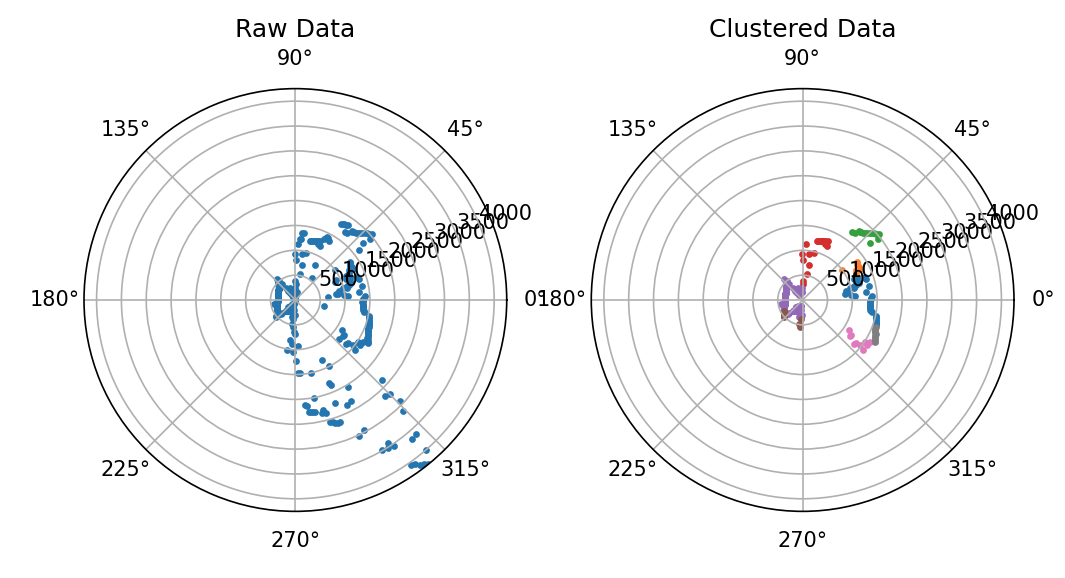
\includegraphics[width=0.5\textwidth]{clusterAccuracy.PNG}
  \caption{DBSCAN Clustering Algorithm}
  \label{fig:dbscan}
\end{figure}

\begin{figure}[h]
\centering
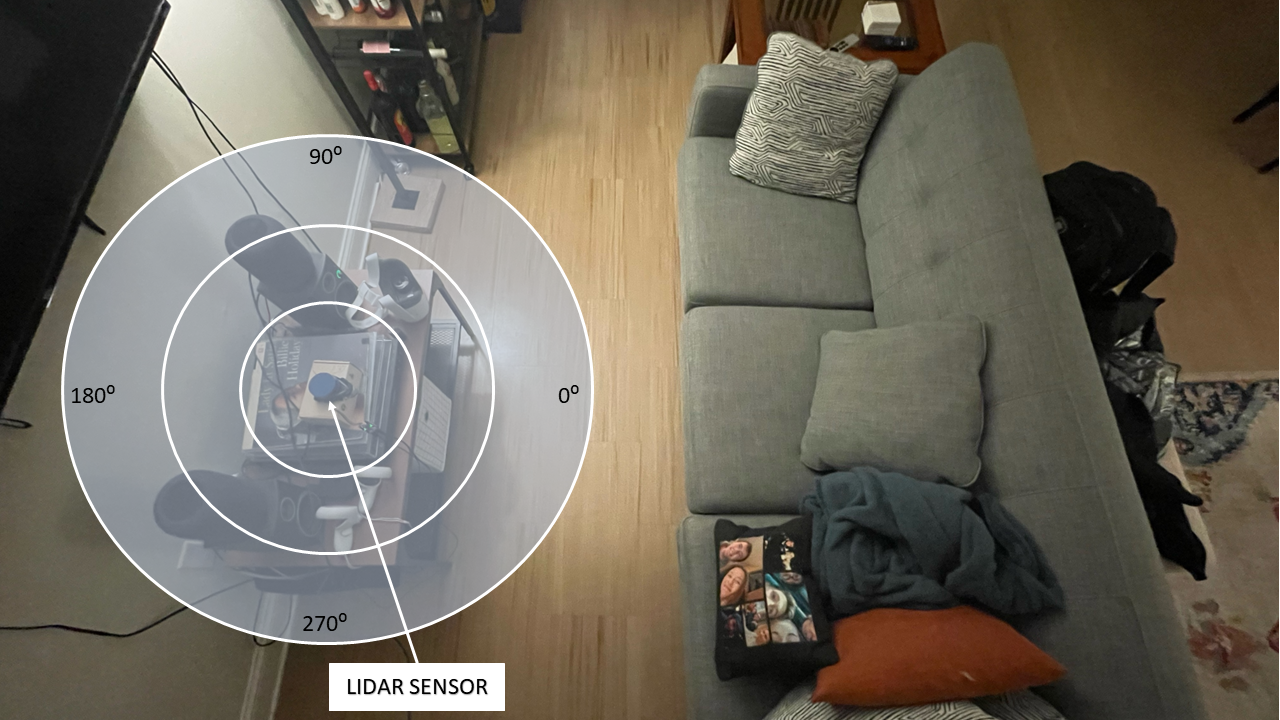
\includegraphics[width=0.5\textwidth]{realWorldScene}
\caption{Real-World Scene}
\label{fig:realworld}
\end{figure}

A noteworthy accomplishment of the DBSCAN clustering was the ability to differentiate between the pillows and the couch itself. The DBSCAN algorithm was very accurate.\\

\subsubsection{Latency and Resource Utilization}

As previously mentioned, due to the nature of the DBSCAN algorithms all points must be visited as a result the latency as reported in the synthesis report is 362 ns. All synthesis reports to include the custom algorithm implemented and attempts at optimizations resulted in a latency of 362 ns. Additionally, the actually latency depends on the AXI DMA stream interface and the specific data as well. The following times collected for the different implementations was performed on the same data set.

\begin{table}[h]
\centering
\begin{tabular}{|c|c c c|}
\hline
\textbf{Algorithm} & \textbf{Software} & \textbf{Custom Algorithm} & \textbf{DBSCAN} \\
 \hline
\textbf{Time (s)} & 0.6659 & 0.0227 & 0.01475 \\
 \hline
\end{tabular}
\caption{Elapsed Times for Different Clustering Implementations}
\label{table:processing_times}
\end{table}

The DBSCAN implementation demonstrated the fastest performance a 97\% decrease over the software benchmark and 35\% decrease over the custom algorithm. The performance gains can likely be attributed to its more stringent clustering criteria. In the DBSCAN clustering algorithm, more points are excluded as they are considered noise, resulting in smaller clusters and consequently, reduced latency from receiving the clusters. The speed improvement compared to the software benchmark can be attributed to several factors, such as the hardware clustering algorithm having more optimized mathematical operations, lower latency compared to Python, and the inherent advantages of using LiDAR operations with large datasets. In such cases, it is beneficial to transfer data between the processing system and programmable logic to enhance performance as we have proven.\\

With respect to resource utilization, the FPGA area for each hardware implementation, which includes Digital Signal Processors (DSPs), Flip-Flops (FF), and Lookup Tables (LUT), was calculated using the following formula:

\[ 
\text{FPGA AREA} = 10 * \text{DSP} + \text{FF} + \text{LUT}
\]

The table presents the FPGA area used by each implementation:

\begin{table}[h]
\centering
\begin{tabular}{|c|c|c|c|c|}
\hline
\textbf{Implementation} & \textbf{DSP} & \textbf{FF} & \textbf{LUT} & \textbf{Area} \\
\hline
Custom & 91 & 20418 & 15924 & 127342 \\
DBSCAN1 & 284 & 36695 & 41829 & 725048 \\
DBSCAN2 & 152 & 18871 & 21544 & 192415 \\
DBSCAN\_LUT & 13 & 3037 & 3827 & 19864 \\
\hline
\end{tabular}
\caption{FPGA Resource Utilization}
\label{table:fpga_resource_utilization}
\end{table}

The DBSCAN\_LUT implementation made the most efficient use of the FPGA fabric, achieving an 84\% area reduction compared to the custom algorithm and a 97\% reduction compared to the first DBSCAN implementation. By employing hard-coded sine and cosine look-up tables and using fixed-point arithmetic, we managed to preserve the mathematical accuracy of the original DBSCAN while significantly decreasing the number of resources needed.


\subsection{Cluster Tracking}
The cluster tracking implementation was not as effective as the DBSCAN clustering algorithm. Evaluating the effectiveness of the cluster tracking is somewhat challenging to convey qualitatively; however, by examining the graphical representation, its accuracy can be assessed. In the graph, the symbol 'X' denotes the centroids stored in the Kalman Filter, and centroids sharing the same color indicate they belong to the same cluster.

Upon analyzing the plots shown in Figure \ref{fig:kalmanFilter}, it is apparent that, although most centroids are accurately positioned, a few outliers are present. This observation suggests that the Kalman Filter parameters warrant further refinement to enhance the performance and accuracy of the cluster tracking process. By fine-tuning these parameters, it is possible to potentially improve the effectiveness of the cluster tracking, resulting in more reliable and precise outcomes.

\begin{figure}[h]
  \centering
  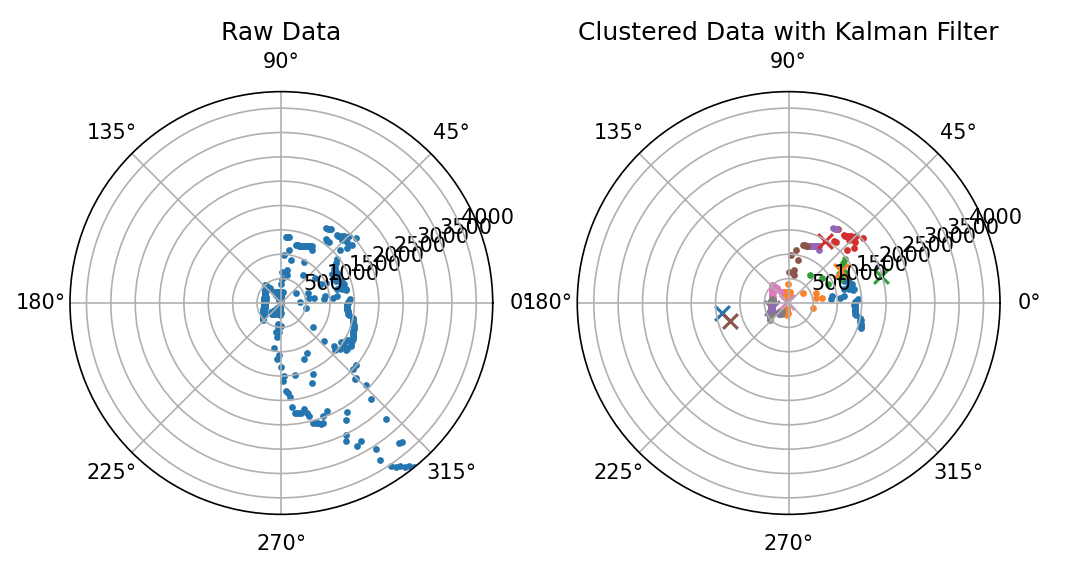
\includegraphics[width=0.5\textwidth]{kalmanFilter.PNG}
  \caption{DBSCAN Clustering Algorithm}
  \label{fig:kalmanFilter}
\end{figure}

\subsection{Challenges}
Several challenges were encountered during the course of this project:

\begin{enumerate}
\item \textbf{Resource Ceiling:}
On multiple occasions, a suitable clustering algorithm or additional HLS optimizations were identified, but they consumed excessive resources. This often led to an extended synthesis duration. In some cases, a resource limitation was not immediately apparent. For example, the cluster IP might be below the DSP ceiling initially, but when additional IPs are incorporated into the FPGA, the overall resource utilization, specifically DSPs, might exceed the acceptable threshold.

\item \textbf{Extremely Slow Plotting:}
An easy method to verify the proper functioning of the clustering algorithm and ensure that clusters are being correctly identified is to graph the data. However, graphing proved to be a time-consuming process, with several minutes elapsing before a plot would appear. This significantly slowed the workflow. This issue became particularly prominent during the data association and Kalman Filter stages of the project, as development required a third graph, which further strained the already burdened system.

\item \textbf{Limitations of Clustering Algorithms:}
One example of such a challenge is the inherent limitations of certain clustering algorithms, such as DBSCAN. This algorithm essentially necessitates visiting each point sequentially while constructing a "path." The presence of data dependencies in this process hinders the potential for parallelism, which in turn obstructs further improvements in latency. The limitations of the clustering algorithms made it difficult to optimize performance and achieve the desired efficiency in processing the data.

\end{enumerate}

\subsection{Improvements}

In order to further enhance the performance and capabilities of the system, several potential improvements have been identified for future exploration. These improvements are aimed at optimizing various aspects of the system, such as reducing latency, increasing resolution, and employing hardware acceleration. The following list provides a brief overview of these potential enhancements:

\begin{enumerate}
\item \textbf{Stream Plots to External Screen:}
One potential solution to address the slow plotting issue is to enable the PYNQ board to export the plots directly to an external monitor via its onboard HDMI interface. By doing so, the latency associated with plotting could be significantly reduced, thereby improving the workflow efficiency.

\item \textbf{Custom Python LiDAR Library:}
The current Python LiDAR library provides a resolution of 1 degree, irrespective of the operating frequency. However, the LiDAR sensor is capable of achieving a 0.5-degree resolution at 7 Hz. Implementing a custom interface between the PYNQ board and the LiDAR sensor could lead to increased resolution and greater control over the LiDAR data collection process, resulting in more accurate and detailed data.

\item \textbf{Additional HLS Optimization:}
There are opportunities to explore further HLS optimizations within the clustering algorithm. Although the current algorithm performs satisfactorily in terms of performance and resource utilization, additional HLS optimizations, such as array indexing, could potentially reduce latency even further and enhance the overall efficiency of the system.

\item \textbf{Migrate Kalman Filter to Hardware:}
The Kalman Filter presents an outstanding opportunity for hardware acceleration, primarily due to its inherent parallelism in matrix operations and computational efficiency. By transitioning the Kalman Filter to hardware, substantial performance enhancements, reduced latency, and more dependable cluster tracking can be attained in real-time applications. This hardware-based approach enables a more efficient and robust implementation, better suited for demanding applications with stringent processing requirements.

\end{enumerate}

\section{Conclusion}

This paper presents an efficient solution for real-time processing and analysis of LiDAR data using FPGA-based hardware acceleration. The proposed approach employs a YDLiDAR X4 LiDAR sensor for data collection and a Xilinx FPGA platform for acceleration, achieving significant improvements in overall performance. The integration of a constant velocity Kalman filter enables accurate tracking of detected clusters over time, while the data visualization using polar plots provides a clear representation of the raw LiDAR data and the identified clusters. The hardware accelearted DBSCAN clustering algorithm saw a 97\% improvement over the the software benchmark and we were successfuly able to track clusters over time using a Kalman filter.

\begin{thebibliography}{00}
    \bibitem{b1} L, Mallidi, "PyLidar3," GitHub, 2020, url: https://github.com/lakshmanmallidi/PyLidar3
    \bibitem{b2} K, Konstantinidis, "Detection and Tracking of Moving Objects with 2D LiDAR," GitHub, 2022, url: https://github.com/kostaskonkk/datmo
    \bibitem{b3} K. Beomseong, C. Baehoon, Y. Minkyun, K. Hyunju, K. Euntai. (2014). Robust Object Segmentation Using a Multi-Layer Laser Scanner. Sensors (Basel, Switzerland). 14. 20400-18. 10.3390/s141120400. 
    \bibitem{b4} R. Su, J. Tang, J. Yuan and Y. Bi, "Nearest Neighbor Data Association Algorithm Based on Robust Kalman Filtering," 2021 2nd International Symposium on Computer Engineering and Intelligent Communications (ISCEIC), Nanjing, China, 2021, pp. 177-181, doi: 10.1109/ISCEIC53685.2021.00044.
    \bibitem{b5} N. Baisa, "Derivation of a Constant Velocity Motion Model for Visual Tracking," arXiv, 2020, doi: 10.48550/ARXIV.2005.00844

\end{thebibliography}

\end{document}
